\chapter{L'optimisation continue} 

\section*{Introduction}

Avant de pouvoir proposer n'importe quel algorithme d'optimisation continue, il faudra d'abord établir une étude comparative entre les différentes approches proposées dans le passé. Cela permet d'élargir notre champ de connaissances en tenant compte des points forts des autres algorithmes et de ne pas reprendre les erreurs commises par les autres chercheurs.

Nous ne pouvons pas présenter toutes les approches proposées auparavant, donc nous nous contentons de le faire pour quelques méta-heuristiques et les domaines dans lesquelles elles ont été appliquées pour l'optimisation continue.
\section{Méta-heuristiques pour les problèmes à variables continues}
\subsection{L'algorithme Particle Swarm Optimization (PSO)}
C'est en 1995 que l'algorithme PSO a été proposé par Kennedy et Eberhart pour traiter les problèmes d'optimisation continue \cite{KENNEDY_EBERHART_1995}.

Cette approche simule les comportements des particules telles que les poissons et les oiseaux migrateurs qui se comportent en fonction du comportement global du groupe.

Du point de vu informatique, les particules représentent les solutions candidates d'une population. Les particules évoluent simultanément par partage d'information avec le voisinage. Le rôle de chaque particule est de générer une solution en se basant sur son vecteur vitesse, puis de chercher à améliorer sa position dans l'espace en modifiant son vecteur vitesse à l'instant $t+1$ grâce à trois critères qui caractérisent son mouvement: \\
\vspace{-2em}

\begin{itemize}
	\item sa propre vitesse à l'instant $t$,
	\item sa meilleure position par le passé,
	\item la meilleure position connue de la population.
\end{itemize}

Il y a trois types de comportements de particules:

\begin{itemize}
	\item égoïste (la particule prend son propre chemin),
	\item conservatif (la particule conserve sa position),
	\item panurgique (la particule suit le meilleur comportement du groupe).\\
\end{itemize}

L'algorithme PSO est le suivant.\bigskip

\begin{algorithm}[H]
	\caption{PSO}
	\KwIn{La condition d'arrêt}
	\KwOut{La meilleure solution trouvée}
  	\Begin{
		Initialisation aléatoire de l'essaim de particules\;
		\While{la condition d'arrêt est non vérifiée}
		{
			$gbest \leftarrow$ meilleur $pbest_i$ de toutes les particules\;
			\For{chaque particule$_i$}
			{
				$v_i^{t+1}\leftarrow w v_i^t + r_1 c_1 (x_i - pbest_i)+r_2 c_2(x_i - gbest)$\;
				Mise à jour de la position de la particule $x_i^{t+1} \leftarrow x_i^t + v_i^{t+1}$\;
			}
			\For{chaque particule$_i$}
			{
				Calculer la valeur de la fonction $fitness$\;
				\If{$fitness < pbest_i$ \tcc{meilleure valeur rencontrée pour la particule}}{
					$pbest_i \leftarrow fitness$\; 
				}
			}
  }
}
\end{algorithm}

\parbox[c][7em][s]{\textwidth}{}

\begin{spacing}{1.6}

PSO a été également développé et appliqué sur un problème de reconfiguration des systèmes de
distribution pour minimiser la perte d'énergie. La méthode proposée
reformule le problème en tant que problème d'optimisation non linéaire.
Elle a été examinée et testée sur les systèmes de test standards IEEE14,
IEEE30 et IEEE118 \cite{esmin2012application}.

\bigskip

Encore, PSO a été appliqué sur un problème de modélisation des
réseaux de transport pour minimiser le temps de voyage tout en
assurant que le budget n'excède pas une certaine limite. PSO a été
comparé avec l'algorithme Hybridized Ant Colony Optimization (HACO) qui a été conçu spécialement pour ce genre de problèmes et a donné de bons résultats \cite{babazadeh2011application}.

\bigskip

Malheureusement, PSO souffre du problème de la convergence prématurée, c'est la raison pour laquelle une version mathématique intégrale modifiée de PSO a été mise au point pour le problème de planification des systèmes de chauffage afin de minimiser le coût du système pour un
cycle de vie donné. Il a été prouvé que la version améliorée de PSO
(improved PSO, IPSO) résout le problème efficacement et fournit des
informations qui montrent qu'il est apte à régler des problèmes de
planification réels \cite{ma2013application}.

\bigskip

\subsection{L'algorithme Bat Algorithm (BA)}
C'est un algorithme bio-inspiré récent, développé par Xin-She Yang en 2010 \cite{yang2010new} pour les problèmes d'optimisation globale. Il est inspiré des écholocations naturelles des chauves-souris qui peuvent trouver et discriminer les différents types d’insectes et éviter les obstacles, même
dans l’obscurité totale.

\bigskip

Cet algorithme se base sur les trois étapes répétitives suivantes:

\bigskip
\begin{itemize}
	\item l'évaluation de la performance de chaque chauve-souris,
	\item la mise à jour des meilleures solutions locales et globales,
	\item la mise à jour de la position, de la vitesse et de la fréquence de chaque chauve-souris. 
\end{itemize}

\end{spacing}

\vspace{-5em}
L'algorithme BA est le suivant.

\bigskip\bigskip

\begin{algorithm}[H]
	\KwIn{Les paramètres de l'algorithme et la condition d'arrêt}
	\KwOut{La meilleure solution trouvée}
	\Begin{
			Définir la fonction objectif $f(x),x=(x_1,...,x_d)^T$\;
			Initialiser la population des chauves-souris $x_i(i=1,2,...,n)$ et la vitesse de chacune des chauves-souris $v_i$\;
			Calculer la fréquence d'impulsion $f_i$ à la position $x_i$\;
			Initialiser les taux d’émissions de pulsation $ri$ et l'intensité $A_i$\;
			\While{$t$ < nombre maximum des itérations}
			{
				Générer de nouvelles solutions par l’ajustement des fréquences,
				et mettre à jour les vitesses et les positions\;
				\If{$rand>r_i$}
				{
					Sélectionner une solution parmi les meilleures solutions\;
					Générer une solution locale autour de la meilleure solution sélectionnée\;
				}
				Générer une nouvelle solution en volant aléatoirement\;
				\If{$rand<A_i$ et $f(x_i)<f(x_*)$}
				{
					Accepter les nouvelles solutions\;
					Incrémenter $r_i$ et réduire $A_i$\;
				}
				Classer les chauves-souris et trouver la meilleure solution courante\;
			}
			Post-traitement des résultats et visualisation\;		
		}
	\caption{BA}
\end{algorithm}

\vspace{3em}
\begin{spacing}{1.6}
La mise à jour des vitesses et des positions des chauves-souris est similaire à celle des particules dans l'algorithme PSO. C'est pour cela que BA est considéré comme une extension de PSO avec une recherche locale contrôlée par l'intensité et par le taux d'émission des ondes.
\end{spacing}

\section{Méta-heuristiques adaptées aux problèmes à \\ \mbox{variables} continues}
\subsection{L'algorithme Ant Colony Optimization pour les domaines continus (ACO$_\mathbb{R}$)}
Initialement proposée en 1991 \cite{dorigo2006ant}, l'approche ACO s'inspire du comportement naturel des fourmis. Ces insectes commencent par une exploration aléatoire de l'espace de recherche, puis déposent de la phéromone en fonction de la quantité et de la qualité de nourriture trouvée. Après une certaine période de temps, la meilleure source de nourriture aura la plus forte concentration de phéromone. Du coup, la colonie de fourmis s'y dirige.

En informatique, l'approche ACO se base sur la construction incrémentale (variable par variable) des solutions. L'ensemble des composants possibles de la solution est défini par le problème. 

A chaque étape de construction, une fourmi fait un
choix probabiliste pour choisir le prochain composant $c_{ij}$ de la solution à
partir de l'ensemble des composants admissibles $N(s^p)$. La règle exacte de ce choix probabiliste varie d'un algorithme à un autre, la meilleure connue est celle de Ant System (AS) \cite{dorigo1996ant}:

$$ p(c_{ij}|s^p) = \frac{\tau^\alpha_{ij}\cdot\eta(c_ij)^\beta}{\sum_{c_{il} \in N(s^p)} \tau^\alpha_{il}\cdot\eta(c_ij)^\beta} \forall c_{ij} \in N(s^P),
$$

où:
\begin{itemize}
	\item $t_{ij}$ est la valeur de phéromone associée au composant $c_{ij}$,
	\item $\eta$ est la fonction de pondération qui associe, à chaque étape de
	construction, une valeur heuristique à chaque composant admissible
	de la solution $c_{ij} \in N(s^P)$,
	\item $\alpha$ et $\beta$ sont des paramètres positifs qui déterminent la relation entre
	l'information de phéromone et l'information heuristique.
\end{itemize}
\bigskip\bigskip
Une extension de l'approche des colonies de fourmis, appelée ACO$_\mathbb{R}$,  a été présentée pour les domaines continus \cite{SOCHA_DORIGO_2006} . 

Dans l'algorithme ACO$_\mathbb{R}$, Socha et Dorigo proposent d'utiliser une distribution de
probabilité continue (qui est une fonction de densité de probabilité,
Probability density function en anglais, PDF) au lieu d'utiliser une distribution de
probabilité discrète dans le processus de décision.

Dans ACO$_\mathbb{R}$, au lieu de choisir un composant $c_{ij}\in N(s^p)$, une fourmi
échantillonne une PDF en utilisant un ensemble de solutions appelé
archive de solutions. Cette archive remplace la table de phéromone dans l'approche ACO combinatoire, et la mise à jour de la phéromone se traduit ici par le rajout et le retrait des solutions de cette archive. 

Initialement, l'archive de solutions contient $k$ solutions
aléatoires ($k$ est un paramètre empirique). Ensuite, à chaque itération, $m$ nouvelles solutions sont
générées, évaluées et ajoutées à l'archive qui sera donc de taille $k+m$ ($m$
étant le nombre de fourmis). L'archive est par la suite triée selon les
qualités des solutions et seulement les $k$ meilleures sont gardées (la taille
de l'archive restera égale à $k$ à la fin de chaque itération).\\

La représentation de l'archive est la suivante:

\begin{figure}[H]
	\centering
	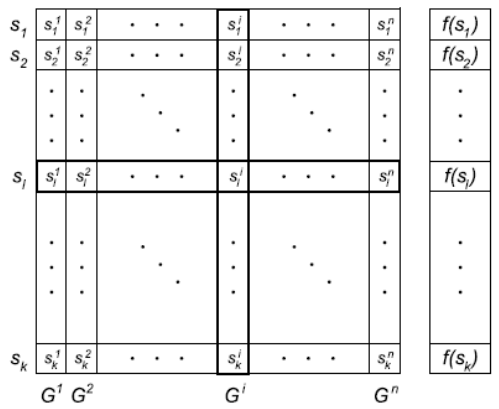
\includegraphics[width=0.65\textwidth,keepaspectratio]{archive}
	\caption{Archive des solutions dans l'algorithme ACO$_\mathbb{R}$}
\end{figure}


\begin{itemize}
	\item $n$ est la taille de la solution (dimension de la fonction problème),
	\item $k$ est le nombre de solutions dans l'archive,
	\item $s^i_l$ est le $i^{ème}$ composant de la $l^{ème}$ solution.
\end{itemize}

Chaque ligne de l'archive correspond à une solution construite par une fourmi. La
qualité de chaque solution est calculée par la fonction objectif et stockée
dans l'archive.

Socha et Dorigo utilisent une fonction de densité de probabilité unidimensionnelle (à une seule variable) et multi-modale basée sur une fonction gaussienne noyau qui représente une somme pondérée de plusieurs fonctions gaussiennes $g^i_l$  où $l$ est l'indice de la solution et $i$ est l'indice du composant. La fonction gaussienne noyau est définie comme suit:

$$
G^i (x) = \sum^{k}_{l=1} \omega_l g_l^i(x) = \sum^{k}_{l=1} \omega_l \frac{1}{\sigma^i_l \sqrt{2\pi}} \mathrm{e}^{-\frac{(x-\mu^i_l)^2}{2\sigma_l^{i^2}}}
,$$

où:
\begin{itemize}
	\item $l \in$ $\{1,...,k\}$,
	\item $i \in$ $\{1,...,n\}$,
	\item $w_l$ est le poids de la $l^{ème}$ solution.
\end{itemize}


Le poids de chaque fonction est calculé selon la fonction gaussienne suivante:

$$
\omega_l = \frac{1}{qk\sqrt{2\pi}} \textrm{e}^{-\frac{(l-1)^2}{2q^2 k^2}}.
$$

Cette formule définit le poids comme étant une valeur de la fonction
gaussienne avec argument $l$, moyenne $\mu=1$ et variance $\sigma=qk$,  où $q$ est un paramètre empirique de l'algorithme.

Lorsque $q$ est petit, les meilleures solutions sont fortement préférées et lorsqu'il est grand, la probabilité devient plus uniforme.

En pratique, dans le processus de construction de solution, chaque composant de la nouvelle solution est traité indépendamment des autres.
Chaque fourmi choisit une des solutions de l'archive selon son poids. La probabilité $p_l$ de choisir la $l^{ème}$ solution est donnée par:
$$
p_l = \frac{\omega_l}{\sum_{r=1}^{k} \omega_r}.
$$

Ensuite, à l'étape $i$, l'algorithme échantillonne la fonction gaussienne associée au $i^{ème}$ composant de la solution choisie en utilisant une fonction
de densité de probabilité gaussienne, avec $\mu^i_l=s^i_l$ et $\sigma^i_l$ donnée par:
$$
\sigma_l^i = \xi \sum_{e=1}^{k} \frac{|S_e^i - S_l^i|}{k-1}.
$$

Cette formule représente la distance moyenne entre la $i^{ème}$ variable de la $l^{ème}$ solution
(solution choisie) et la $i^{ème}$ variable des autres solutions de l'archive,
multipliée par un paramètre $\xi$.

Ce paramètre a un effet similaire à celui du taux d'évaporation de la phéromone dans l'approche ACO. Plus $\xi$ est grand, plus la vitesse de convergence de l'algorithme est petite.

Après le calcul de $\mu^i_l$ et $\sigma^i_l$, la $i^{ème}$ variable de la nouvelle solution aura comme valeur un nombre aléatoire généré en obéissant à la loi gaussienne $N(\mu^i_l,\sigma^i_l)$.  

Le processus de construction de solution est répété $m$ fois pour chaque
dimension $i=1,...,n$ du problème. Après chaque construction de solution, la mise à jour
de la phéromone est traduite par le fait d'ajouter $m$ nouvelles solutions
générées à l'archive $T$ et d'éliminer le même nombre de plus mauvaises solutions; on garde donc le même nombre $k$ de solutions dans l'archive. Ce
processus permet de ne garder que les $k$ meilleures solutions, ce qui va
permettre de bien guider les fourmis dans leur processus de recherche.

L'algorithme ACO$_\mathbb{R}$ permet d'ajouter des activités qu'une simple
fourmi ne peut pas faire: recherche locale sur les solutions construites, récolte d'une information globale pour décider s'il est utile de déposer
encore de la phéromone, etc... Cependant, ces activités n'ont pas été appliquées par Socha et Dorigo.

Le pseudo code de l'algorithme ACO$_\mathbb{R}$ est donné comme suit:\\

\begin{algorithm}[H]
	\KwIn{$k$,$m$,$n$,$q$,$\xi$ et la condition d'arrêt}
	\KwOut{La meilleure solution trouvée}
	\Begin{
	Initialiser et évaluer $k$ solutions\;
	\tcp{Trier les solutions et les mettre dans l'archive}
	$T = Trier(S_1 ... S_{k})$\;
	\While{la condition d'arrêt est non vérifiée}{
		\tcp{Générer $m$ nouvelles solutions}
		\For{$l=1$ \KwTo $m$}{
			\tcp{Construire une solution}
			\For{$i=1$ \KwTo $n$}{
				Choisir une fonction gaussienne $g^i_j$ selon les poids\;
				Échantillonner la fonction $g^i_j$ avec le paramètre $\mu^i_j \cdot \sigma^i_j$\;
			}
			Sauvegarder et évaluer la solution générée\;
		}
		\tcp{Trier les solutions et choisir les $k$ meilleures}
		$T = Meilleure(Trier(S_1 ... S_{k+m}),k)$\;
	}
}
\caption{ACO$_\mathbb{R}$}
\end{algorithm}



\subsection{L'algorithme ACO$_\mathbb{R}$ avec la théorie des perspectives (\mbox{ACO$_\mathbb{R}$-PT})}
Riadi Indra \cite{riadi2014cognitive} a proposé une amélioration de l'algorithme ACO$_\mathbb{R}$ qui garde le même principe que celui de ACO$_\mathbb{R}$ sauf qu'elle modifie la transition d'état lors de la phase de construction. Une solution n'est pas choisie en se basant sur son poids seulement, mais aussi sur son évaluation. C'est pourquoi Indra commence par calculer un point de référence qui est la moyenne des évaluations des solutions de l'archive.

$$point~de~référence = moyenne (f(s_1),f(s_2),...,f(s_k)).$$

Ensuite, il commence à séparer les solutions de l'archive en deux groupes. Les solutions qui ont une évaluation plus petite que celle du point de référence auront un gain négatif par rapport à l'écart du point de référence et les solutions qui ont une évaluation plus grande ou égale à celle du point de référence auront un gain positif.

De plus, une valeur probabiliste est calculée pour chaque solution. Le nouveau poids (perspective) de la solution est obtenu par la multiplication de son gain par sa valeur probabiliste.

La meilleure solution est celle qui a le poids le plus élevé et qui va donc être utilisée pour calculer la nouvelle valeur de phéromone.

\subsection{L'algorithme Continuous Ant Colony Optimization (CACO)}

Cet algorithme, développé par Bilchev et Parmee \cite{bilchev1995ant}, représente le premier essai pour adapter un algorithme inspiré du comportement des fourmis aux problèmes d'optimisation continue. Dans CACO, les fourmis commencent à partir d'un point appelé $nid$, situé quelque part dans l'espace de recherche. Les bonnes solutions trouvées sont stockées en tant qu'ensemble de vecteurs et proviennent du nid. A chaque itération, les fourmis font un choix probabiliste sur un des vecteurs. Ensuite, elles continuent la recherche à partir du vecteur choisi en faisant des mouvements aléatoires. Les vecteurs sont mis à jour par les meilleurs résultats trouvés. 

Bien que les auteurs de CACO prétendent qu'ils se sont inspirés de l'approche ACO originale, CACO présente plusieurs différences avec ACO. En effet, la notion de $nid$ n'existe pas dans l'approche ACO. De plus, CACO ne fait pas une construction incrémentale des solutions alors que celle-ci est l'une des caractéristiques principales de ACO. Donc, CACO n'est pas une extension de ACO.  

\subsection{L'algorithme Continuous Interacting Ant Colony (CIAC)}

Cette approche, basée sur le comportement des fourmis, a été présentée par Dréo et Siarry \cite{dreo2004continuous}. CIAC utilise deux types d'interaction entre les fourmis, l'information stigmergique (points de phéromone déposés dans l'espace de recherche) et la communication directe entre les fourmis. Ces dernières font des mouvements stratégiques en suivant la phéromone et en communicant entre elles. De même que CACO, CIAC n'est pas une extension de ACO car il ne construit pas les solutions de façon incrémentale et est basé sur une communication directe entre les fourmis.

\subsection{L'algorithme Taboo Search (TS)}
La première adaptation de la recherche Tabou aux domaines continus est présentée par Cvijovic et Klinowski en 1995 \cite{cvijovic1995taboo}. Dans cet algorithme, les auteurs ont introduit une structure de voisinage pour l'espace continu qu'ils ont appelée \emph{voisinage conditionnel}. L'espace de solutions $S$ (qui représente un hyper-cube dans $\mathbb{R}^n$, où n est le nombre de variables) est partitionné en des cellules disjointes en divisant en $p_1, p_2,...,p_n$ partitions, les intervalles de coordonnées au long des axes $x_1, x_2,...,x_n$ .

A chaque itération, $n_s$ points sont tirés à partir de $n_c$ partitions choisies au hasard en utilisant une distribution uniforme. Ces points vont constituer les voisins de la solution courante $s^*$. La taille du voisinage $N(s^*)$ est égale à $n_c n_s$.

\subsection{L'algorithme Continuous Tabu Search (CTS)}
Une autre extension de la recherche Tabou proposée par Siarry et Berthiau \cite{siarry1997fitting} explore la notion de voisinage inventée par N. Hu \cite{Hu_1992} qui se base sur le principe de disques centrés par la solution.

\begin{figure}[H]
	\centering
	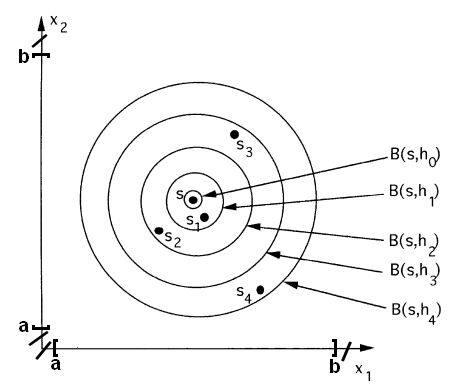
\includegraphics[width=0.45\textwidth,keepaspectratio]{partitionnement_voisinage}
	\caption{Partitionnement du voisinage d'une solution dans CTS}
\end{figure}

Les voisins de la solution sont pris chacun d'une couronne qui sépare les frontières de deux disques consécutifs. Une explication détaillée de cette notion sera expliquée dans le prochain chapitre.

CTS commence à partir d'une solution aléatoire, puis génère un certain nombre fixe de voisins et continue avec le meilleur voisin, même si son évaluation est pire que celle de la solution courante (voisinage en anneau).

Pour éviter de boucler sur les mêmes voisins, chaque voisin généré est inséré dans une liste Tabou circulaire qui garde trace des dernières solutions rencontrées vers lesquelles nous ne devons pas revenir. Cependant, ce processus risque de contourner des mouvements utiles, ce qui nécessite l'incorporation d'un mécanisme d'aspiration qui permet d'éviter une telle situation.  

L'algorithme s'arrête lorsqu'il trouve l'optimum ou lorsqu'il n'arrive pas à améliorer la solution au bout d'un certain nombre d'itérations.
 
\subsection{L'algorithme Enhanced Continuous Tabu Search (ECTS)}
C'est une adaptation de la recherche Tabou aux domaines continus qui consiste d'abord à faire une diversification pour détecter les régions prometteuses, puis à effectuer une intensification afin de trouver l'optimum dans la région la plus prometteuse \cite{Chelouadh_siarry_2001} .

Le voisinage est défini de la même manière que dans CTS sauf que les auteurs ici considèrent des hyper-rectangles au lieu des disques. 

L'algorithme ECTS est le suivant:\\

\begin{algorithm}[H]
	\KwIn{Les paramètres de l'algorithme et la condition d'arrêt}
	\KwOut{La meilleure solution trouvée}
	\Begin{
		Diversification\; 
		Chercher la région la plus prometteuse\;
		\While{la condition d'arrêt est non vérifiée}{
			Intensification\;
			Mise à jour de la meilleure solution\;
		}
	}
	\caption{ECTS}
\end{algorithm}
\bigskip

\subsection{L'algorithme Continuous Reactive Tabu Search (CRTS)}
\begin{spacing}{1.4}
Une amélioration de la recherche Tabou pour les domaines continus a été proposée par Battiti et Tecchiolli \cite{battiti1996continuous}, et qui s'inspire de l'approche combinatoire Reactive Tabu Search (RTS) en la combinant avec un minimisateur stochastique. Le composant combinatoire sert à localiser les régions prometteuses (qu'ils ont appelées boîtes) à partir desquelles le minimisateur effectue sa recherche locale. La taille des boîtes ainsi que les paramètres de recherche sont adaptés automatiquement à la structure locale de la fonction objectif.\\[2em]
\end{spacing}

Les auteurs ont développé une fonction d'évaluation des boîtes qui permet d'indiquer si la boîte contient de bonnes solutions. Ils ont testé deux méthodes de calcul et ont exprimé chacune dans un algorithme:
\begin{itemize}
	\item CRTS$_{average}$ (CRTS$_{ave}$) qui considère la moyenne des évaluations des solutions dans la boîte:
	$$X_i: f(B)\equiv \left(\frac{1}{N_B}\right)\sum_{i=1}^{N_B}f(X_i),$$ où $N_B$ est le nombre de points.
	\item CRTS$_{minimum}$ (CRTS$_{min}$) qui considère le minimum des évaluations des solutions dans la boîte:
	$$f(B)\equiv min_{i\in(1,...,N_B)} f(X_i).$$
\end{itemize}


\subsection{L'algorithme Continuous Genetic Algorithm (CGA)}
L'algorithme génétique se base sur les opérateurs suivants:

\begin{itemize}
	\item la sélection des individus qui doivent se reproduire par la technique de tirage à roulette ou par tournoi ou par rang,
	\item le croisement des individus sélectionnés,
	\item la mutation (modification aléatoire) des nouveaux individus,
	\item le remplacement des parents par les nouveaux individus.
\end{itemize}

La nouvelle population sera construite des meilleures individus de la population courante.
 
La version continue de l'algorithme génétique redéfinit les opérateurs de croisement et de mutation en tenant compte de la taille et de la distribution de la population dans l'espace de recherche \cite{Chelouadh_siarry_2000}.

La taille de la population est initialement large pour une meilleure convergence de l'algorithme, mais elle sera réduite au fur et à mesure pour éviter une explosion en termes de temps d'exécution. De plus, pour une meilleure exploration de l'espace de recherche, la population initiale est construite par des solutions suffisamment éloignées les unes des autres et une solution n'est choisie que lorsqu'elle n'appartient à aucun voisinage des autres solutions de la population.

Les auteurs, comme N. Hu\cite{Hu_1992}, utilisent le principe de disque pour explorer le voisinage d'une solution.

L'algorithme CGA est le suivant:\\

\begin{algorithm}[H]
	\KwIn{La condition de convergence}
	\KwOut{La meilleure solution trouvée}
	\Begin{
		Définir la fonction coût, le coût et les variables\;
		Choisir les paramètres de l'algorithme\;
		\While{la condition de convergence est non vérifiée}{
			Choisir les parents\;
			Croisement\;
			Mutation\;
		}
	}
	\caption{CGA}
\end{algorithm}

\subsection{L'algorithme Enhanced Simulated Annealing (ESA)}
Cet algorithme développé par Siarry et ses camarades \cite{siarry1997enhanced}, manipule les problèmes de grande taille en faisant une discrétisation des variables. La recherche aléatoire itérative est remplacée ici par une exploration de plusieurs espaces euclidiens.

\vspace{1em}

Cet algorithme a été prouvé efficace pour résoudre les problèmes de taille 2 à 200 variables. 

\subsection{L'algorithme Evolutionary Strategies (ES)}
Différentes adaptations de l'algorithme évolutionniste ES aux domaines continus ont vu le jour à travers les années.
\begin{itemize}
	\item (1+1)ES \cite{kern2004learning} se base sur un seul parent qui génère une progéniture par itération. Seul l'individu représentant la meilleure solution est gardé.
	\item Cumulative Step Size Adaptation (CSA-ES) \cite{hansen2003reducing} contrôle la taille du pas global en utilisant un chemin traversé par la population parente à travers un certain nombre de générations,
	\item Covariance Matrix Adaptation (CMA-ES) \cite{hansen2003reducing} est une variante de CSA-ES avec une adaptation aléatoire de la matrice de covariances.
	
\end{itemize}

\subsection{L'algorithme Iterated Estimation of Distribution \\Algorithm (IDEA)}
C'est une adaptation de Estimation of Distribution Algorithms (EDAs) pour les problèmes d'optimisation continue, développée par Bosman et Thierens en 2002 \cite{bosman2002multi}. Pour estimer la distribution de la population parente, IDEA exploite le fait que chaque probabilité jointe multi-variée peut être exprimée en tant que factorisation conditionnelle:
$$
P(x_i,...,x_n)=\prod_{i=1}^{n}P(x_i|x_{i+1},x_{i+2},...,x_n).
$$

Le modèle probabiliste de la population parente est reconstruit à chaque itération.

\subsection{L'algorithme Mixed Bayesian Optimization Algorithm  (MBOA)}
Cet algorithme développé par Ocenasek et Schwarz \cite{ocenasek2002estimation}, est basé sur un réseau bayésien avec des structures locales sous forme d'arbres de décision qui capturent les dépendances mutuelles entre les individus parents. MBOA est une extension continue de l'algorithme hierarchical BOA initialement conçu pour le domaine binaire. MBOA peut traiter les variables de type mixte (discret et continu).

\subsection{L'algorithme INTEROPT}
C'est une méthode numérique conçue par Bilbro Griff et Snyder Wesley  \cite{bilbro1991optimization}, pour optimiser les fonctions non-convexes. Elle est basée principalement sur l'approche du recuit simulé mais traite les problèmes à variables continues. La méthode est complètement générale et capable de résoudre les problèmes qui ont une grande taille.

\vspace{-1em}

\section*{Conclusion}
Chaque méta-heuristique a ses avantages et ses inconvénients. La stratégie de recherche diffère d'un algorithme à un autre mais le but est toujours le même, c'est d'essayer d'arriver à la meilleure solution au problème dans les meilleurs délais possibles.
 
Nous avons présenté deux catégories de méta-heuristiques, celles conçues pour des problèmes à variables continues et celles développées à l'origine pour des problèmes à variables discrètes et qui ont été transformées pour s'adapter aux problèmes à variables continues. Le chapitre suivant est consacré à l'algorithme Bee Swarm Optimization (BSO) et à notre propre adaptation de ce dernier aux problèmes d'optimisation continue.

